\documentclass[12pt, letterpaper]{book}
\usepackage[T1]{fontenc}
\usepackage[italian]{babel}
\usepackage{hyphenat}
\hyphenation{mate-mati-ca recu-perare}
\usepackage{hyperref}
\usepackage{graphicx}

\title{Documentazione}
\author{Benedetta Vitale - Emilio Meroni}
\date{\today}

\graphicspath{{../../Immagini}}

\begin{document}

\maketitle

\tableofcontents

\chapter{Project Plan}

\section{Introduzione}

Questo progetto verrà svolto da Benedetta Vitale ed Emilio Meroni, entrambi studenti al terzo anno d'ingegneria informatica presso l'università di Bergamo.\\

Il software che andremo a sviluppare è pensato per dare supporto
all'attività di ristorazione. In particolare, dovrà assistere alle mansioni dei camerieri, come ad esempio: prendere le ordinazioni, redigere il conto, trovare i tavoli disponibili, ecc.\\

Abbiamo scelto questa tipologia di sistema dato che Emilio lavora, nei week-end, presso un ristorante, e gli ha incuriosito la gestione interna tramite l'utilizzo dei palmari da parte dei camerieri.
\begin{tabbing}

\end{tabbing}

\section{Modello di Processo}

Il modello di processo che seguiremo è quello della prototipazione, in particolare la prototipazione evolutiva [Figura: \ref{fig: modello_processo_evolutivo}]. Questo processo è molto utile per quanto riguarda la costruzione dell'interfaccia grafica, dato che ci aiuterà a costruire più velocemente la GUI finale, tramite diversi prototipi d'interfacce utente. La parte principale della nostra applicazione, infatti, sarà la grafica.

\begin{figure}[h]
    \centering
    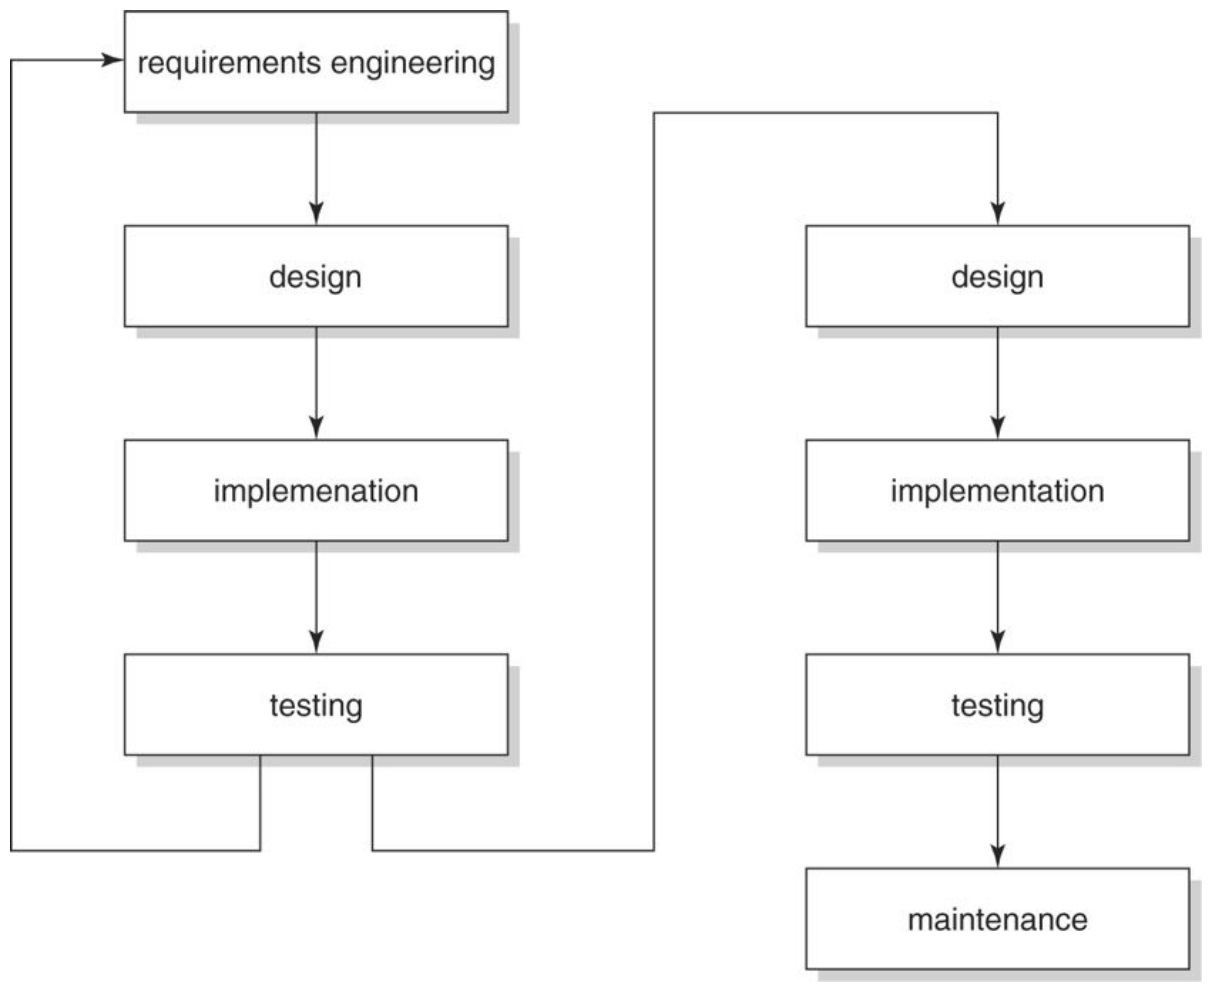
\includegraphics[width = 0.7\linewidth]{../../Immagini/Modello_Processo_Evolutivo.jpg}
    \caption{Modello Di Processo Evolutivo}
    \label{fig: modello_processo_evolutivo}
\end{figure}

\section{Organizzazione del Progetto}\label{sez: organizzazioneProgetto}

Utilizzeremo una organizzazione a tre livelli:

\begin{enumerate}
    \item Data Base
    \item Logico
    \item Presentazione
\end{enumerate}
Il livello \textit{Data Base}, come da nome, si occuperà della parte del DB, il quale sarà embedded.

Il livello \textit{Logico}, possiamo posizionarlo graficamente tra il livello Data Base e quello Presentazione. Funge da intermediario tra i due livelli e fornisce gli oggetti principali per la gestione dell'applicazione.

L'ultimo livello, quello di \textit{Presentazione}, sarà quello visto dall'utente che usufruirà dell'applicazione. Possiamo definirlo come il livello più esterno dove i dati verranno presentati in modo grafico e, la gestione dei tavoli e delle comande sarà fatta in modo interattivo.\\

Il progetto verrà suddiviso in:
\begin{itemize}
    \item \textbf{Documentazione}; questa parte verrà svolta da entrambe le figure coinvolte nel progetto.
    \item \textbf{Progettazione desing}; parte eseguita da Benedetta, che apprezza particolarmente questo ambito.
    \item \textbf{Codifica desing}; questa porzione verrà eseguita principalmente da Emilio, dato che ha una maggiore esperienza sulla programmazione.
    \item \textbf{Codifica parte logica} e \textbf{data base}; le quali verranno scritte sia da Benedetta e sia da Emilio.
\end{itemize}

\section{Standard, Linee guida, Procedure}

Per la parte della stesura della documentazione si è scelto di utilizzare un tool molto utile nella scrittura di documenti professionali, \textit{LaTeX}. Scelta quasi obbligata, derivata dall'utilizzo di \textit{GitHub} insieme al programma di scrittura precedente \textit{Microsoft Word}; il quale ha causato difficoltà nei "merge" su \textit{GitHub}.\\

Mentre, per la parte di \textit{codifica} abbiamo scelto di utilizzare lo standard definito da \textit{Java}\footnote{Standard di Java si possono trovare su questo \href{https://www.oracle.com/java/technologies/javase/codeconventions-contents.html}{\underline{sito}}}. In primo luogo perché l'IDE utilizzato per la parte di programmazione è \textit{Eclipse}, il quale fornisce strumenti per la formattazione e nominazione di metodi in modo automatico secondo gli standard di \textit{Java}; inoltre, non avendo entrambi molta esperienza ci è venuto comodo utilizzare uno dei pochi standard di codificha che conosciamo.\\

Lo strumento che utilizzeremo per la condivisione della documentazione e del codice sarà, come già anticipato, la piattaforma di condivisione \textit{GitHub}.

\section{Attività di Gestione}

La priorità fissata per questo progetto sarà quella di avere una documentazione dettagliata, e, specialmente, di avere un project plan completo per l'inizio del mese di dicembre. Parellamente alla stesura di quest'ultimo si è deciso di dedicare, almeno una volta a settimana, del tempo sulla parte di progettazione.


\section{Rischi}

In questa sezione si discutono i rischi che potrebbero verificarsi durante lo sviluppo del progetto.

Un primo rischio, evidenziato da entrambe le parti, sono le difficoltà che potrebbero verificarsi nell'utilizzo di \textit{windows builder} (plugin che consente la costruzione dell'interfaccia utente su \textit{Eclipse}), dovuta a una bassa conoscenza del tool. Un probabile "effetto" sarà quello di allungare i tempi di codifica sul modulo di presentazione.

\section{Personale}
Il numero di persone che lavoreranno a questo progetto sarà molto ristretto, nello specifico sono:
\begin{itemize}
    \item Benedetta Vitale
    \item Emilio Meroni
\end{itemize}
I quali participeranno in modo equo a quasi tutte le attività. Si è deciso che si lavorerà spesso in coppia, in particolar modo sulla parte di programmazione della GUI, dato che la parte grafica su \textit{Java} non è mai stata approfondita da entrambe le parti, e questo progetto ha una parte di grafica molto importante.


\section{Metodi e Tecniche}

Per ogni nuova modifica aggiunta al progetto, prima di eseguire il "merge" su \textit{GitHub}, la verificheremo tramite dei test. Sulla parte grafica il test verrà eseguito in modo visivo, tramite l'esecuzione del programma.
Se questo funzionerà ancora si procederà con l'aggiunta di nuove modifiche, così da avere sempre un codice eseguibile.

\section{Garanzia e Qualità}

Il programma dovrà essere utilizzato in ristoranti, e in particolare, dal personale che prenderà le ordinazioni. Quindi dovrà essere di \textit{facile} utilizzo, con un focus maggiore sulla funzionalità che sull'estetica. Un'altra qualità che dovrà garantire è la \textit{prevenzione di errori} da parte degli utenti, come ad esempio il "miss-click" (click errati o accidentali).\\

In particolare abbiamo evidenziato quattro qualità che il sistema dovrà possedere:

\begin{enumerate}
    \item \textbf{Semplice}: Il programma sarà scritto per avere poche sezioni scritte e di facile comprensione, anche per chi si approccia al programma per la prima volta. Si utilizzeranno poche schermate che contengono tutto il necessario per le \textit{macro} operazioni definite.
    \item \textbf{Intuiblile}: L'utilizzo dei colori per indicare gli stati dei \textit{tavoli}, in particolare si è deciso che: per i \textit{tavoli liberi} si utilizzerà il colore verde, per i \textit{tavoli occupati} il colore rosso e per i \textit{tavoli da pulire} l'arancione [Figura: \ref{fig: es_bottoni}].
    \item \textbf{Prevenzione Errori}: Per la prevenzione degli errori si utilizzeranno schermate \textit{pop-up}, per la convalida degli input.
    \item \textbf{Veloce}: Con questo termine si indica che il programma, che verrà utilizzato da dispositivi touch, dovrà essere principalmente composto da bottoni che minimizzano i tempi di utilizzo, puntando a un uso minimo della tastiera. Comportando un'esperienza più agevole per l'utente.
\end{enumerate}

\begin{figure}[h]
    \centering
    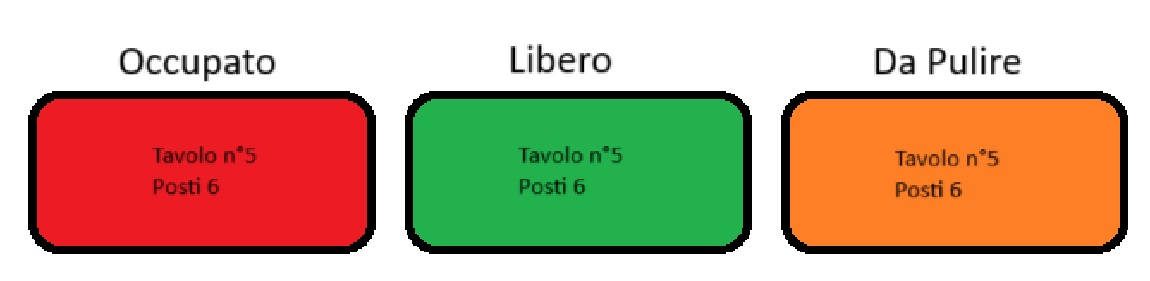
\includegraphics[width=0.6\linewidth]{Esempio_Bottoni.jpg}
    \caption{Esempio di colorazione dei bottoni per i tavoli}
    \label{fig: es_bottoni}
\end{figure}


\section{Workpackages}

I moduli presenti in questo progetto, come già anticipato parzialmente nella sezione \ref{sez: organizzazioneProgetto}, saranno:
\begin{itemize}
    \item \textbf{Documentazione}
    \item \textbf{Codifica desing}
    \item \textbf{Codifica parte logica}
    \item \textbf{Codifica data base}
\end{itemize}

L'organizzazione dei pacchetti di lavoro, presenti su \textit{GitHub}, sarà suddivisa in cartelle, per la parte di codifica raggrupperemo i diversi moduli in unico folder; mentre, la documentazione sarà posizionata in una cartella a parte.\\

Oltre ad avere queste directory, si avrà una parte dedicata ai modelli \textit{ER}(riguardanti il data base) e una per la parte \textit{UML} contenente tutti grafici per la progettazione.

\section{Risorse}

Gli strumenti che verranno adottati in questo progetto saranno:
\begin{itemize}
    \item Per la parte di \textbf{codifica}, come già detto in precedenza, l'IDE \textit{Eclipse}, uno strumento specifico per la scrittura di codice e gestione di progetti \textit{Java}.
    \item In \textbf{scrittura} si utilizzerà l'editor di testo open source \textit{VS Code}, con l'estensione \textit{LaTeX Workshop}, per la scrittura di documenti in formato \textit{LaTeX}. Contribuendo garantire una presentazione accurata dei documenti.
    \item Infine, riguardo agli strumenti di \textbf{Software Configuration Management}, adotteremo \textit{GitHub}. Questa piattaforma sarà impiegata principalmente per la condivisione, gestione e tracciamento delle modifiche al software, oltre che per la documentazione.

\end{itemize}

\section{Budget}

Per quanto riguarda il budget, si è previsto un tempo totale di 80 ore lavorative. Con una forte attenzione sulla parte di documentazione (comprendendo anche la parte di documentazione del codice), rispetto a quella di codifica.\\

In prima approssimazione possiamo definire una divisione del tempo come mostrato in figura [\ref{fig: diagramma_gant}].
\begin{figure}[h]
    \centering
    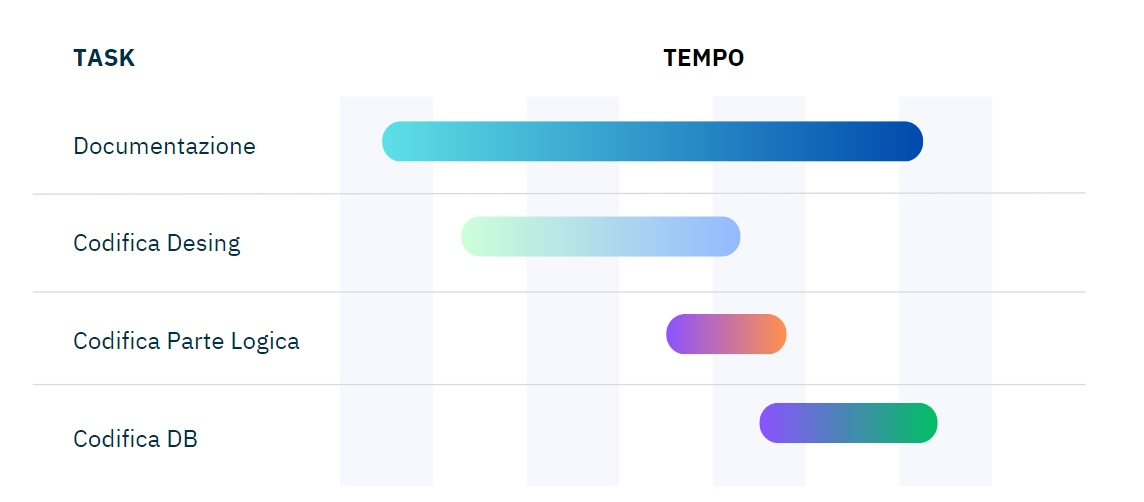
\includegraphics[width = 1\linewidth]{Diagramma_Gant.jpg}
    \caption{Diagramma di Gant}
    \label{fig: diagramma_gant}
\end{figure}

\section{Cambiamenti}

Per quanto riguarda le modifiche che verranno richieste si seguirà la seguente scaletta: inizialmente si verificherà la fattibilità, in caso negativo si cercheranno altre soluzioni che vadano incontro al cliente. Mentre, se si accettano, verrà creato un "branch" sulla piattaforma di \textit{GitHub}. Da qui si aggiornerà la documentazione e i vari diagrammi \textit{UML}, in seguito si procederà alle modifiche del codice. Infine prima di eseguire il "merge" delle modifiche con il \textit{main branch}, si eseguiranno dei test di verifica della funzionalità e di correttezza.

\section{Consegna}


In questa sezione si discutono i metodi e le scadenze di consegna del progetto, in particolare la consegna si dividerà in due fasi:


\begin{itemize}
    \item Consegna del \textbf{Project Plan}, il quale dovrà essere consegnato circa un mese prima del primo esame scritto, che si svolgerà nel mese di gennaio; quindi, per il mese di dicembre si dovrà effettuare la prima consegna.
    \item Consegna del \textbf{Progetto}, quest'ultimo avrà una scadenza più lunga, infatti, l'ultimo giorno di consegna sarà cinque giorni prima dell'esame orale.
\end{itemize}
Per quanto riguarda i metodi di consegna si dovrà condividere con il professore Gargantini la repository di \textit{GitHub} contenente il progetto. Per la consegna della documentazione si dovrà indicare nel file \textit{readMe}, della repository, la posizione del project plan. Mentre, per la consegna del progetto si dovrà creare un \textit{issue}, intitolata “Approvazione Progetto” e assegnarla al professore.

\chapter{Specifiche dei Requisiti}

\section{Introduzione}
\subsection{Obiettivo}
L'obiettivo di questa applicazione sarà quello di diminuire i tempi di ordinazione aiutando  il personale in sala con la gestione delle comande.
\subsection{Scopo}
Questa applicazione principalmente dovrà prendere ordinazioni e calcolare l'importo totale. Avere una organizzazione dei tavoli sapendo in qualsiasi momento lo stato di essi. avendo anche la possibilità (ad inizio o fine giornata) di modificare tutti i servizi che dispone per una maggiore organizzazione ai futuri cambiamenti che il ristorante adotterà all'interno di esso (es aggiunta di tavoli, di menù , ecc.)
\subsection{Definizione del dizionario}
\begin{itemize}
    \item \textbf{Componenti}: sono sezioni di menù nei quali, al loro interno, contengono le diverse pietanze per quella specifica componente. Ad esempio: la pietanza “spaghetti alla carbonara” si trova all'interno della componente “primi”.
    \item \textbf{Caposala}: persona che può accedere anche alle modifiche, cioè alle impostazioni, oltre alle funzioni classiche dell'applicazione.
    \item \textbf{Cameriere}: persona che può solo utilizzare l'app senza accedere alle impostazioni
\end{itemize}
\section{Descrizione Globale Del Sistema}
\subsection{Funzioni del prodotto}
In questa sezione descriviamo le funzioni che gli utenti potranno fare:
\begin{enumerate}


    \item \textbf{Occupazione dei tavoli}: l'utente seleziona un tavolo libero e segnalerà il numero delle persone che si siederanno.
    \item \textbf{Segnalazione Tavolo Da Pulire}: l'applicazione dovrà segnalare se un tavolo è ancora da pulire, e se verrà pulito, l'utente potrà indicare che il tavolo è pulito.
    \item \textbf{Prendere le ordinazioni}: l'utente entrerà nel tavolo occupato e inizierà a prendere le varie ordinazioni scegliendo tra le diverse componenti. Potrà inserire commenti per ciascun piatto, aumentare la quantità per portata ed eliminare dei piatti aggiunti.
    \item \textbf{Inviare gli ordini}: L'invio è il momento che renderà l'ordine immutabile e che lo renderà visibile alla cucina.
    \item \textbf{Segnalare Pagamento effettuato}: l'utente entrerà nel tavolo occupato e, dopo che i clienti avranno pagato, potrà segnalare che il pagamento è stato effettuato.
    \item \textbf{Impostazioni}: Questa sezione dovrà essere accessibile solo da dei caposala.
          \begin{itemize}
              \item \textbf{Modificare la sala}: la modifica della sala comprende operazioni di modifica dei nomi e posti a sedere, l'eliminazione e l'aggiunta dei tavoli.
              \item \textbf{Modifiche piatti e componenti}: Questa funzione servirà a modificare, aggiungere ed eliminare componenti e piatti:
              \item \textbf{Piatti}: si considereranno modifiche sia sul nome sia sul prezzo
              \item \textbf{Componenti}: Modifica del nome della componente
              \item \textbf{Modificare il prezzo del coperto}: si potrà modificare il prezzo che si desidererà per il coperto.
          \end{itemize}
\end{enumerate}
\subsection{Caratteristiche dell'utente}
Gli utenti saranno il cameriere e il caposala, i quali potranno accedere all'applicazione per assegnare tavoli, prendere ordinazioni e cambiare stato del tavolo. Solo il caposala, inoltre, potrà accedere alla sezioni delle impostazioni, nella quale potrà modificare la quantità dei tavoli, delle componenti, dei piatti e il costo del coperto.

\subsection{Vincoli}
Di seguito elenchiamo i vincoli che dovranno esserci:
\begin{itemize}
    \item L'utente cameriere non potrà accedere alle impostazioni.
    \item Le caratteristiche di un tavolo potranno essere modificate solo quando il tavolo sarà nello stato di libero.
\end{itemize}



\section{Requisiti specifici}
\subsection{Requisiti Interfacce utente}
\subsubsection{Generale}
All'apertura si ha un interfaccia scorrevole con le diverse icone dei tavoli, con il nome e il numero dei posti del tavolo. Il tavolo è colorato di rosso se è occupato, di verde se è libero e di arancione se deve essere pulito.
In ogni schermata rimane sempre: in alto a destra i pulsanti “Impostazioni” e “Chiudi”, in alto a sinistra un pulsante “Tavoli” per ritornare alla pagina principale dei tavoli.
\subsubsection{Colorazione Tavoli}
Se il tavolo è verde, il cameriere potrà schiacciarlo dove si aprirà una schermata pop-up in cui inserisce il numero di coperti (quindi ci sarà un pulsante in cui c'è il numero al centro, in basso il “+” e in alto il “-”; si può aggiungere il numero dei coperti finché non si raggiunge il numero dei posti massimi selezionati per quel tavolo) e salvandolo tramite il pulsante “salva” il tavolo diventa rosso. Mentre se il tavolo che ha schiacciato era arancione si aprirà una schermata pop-up dove ci sarà un tasto con su scritto “pulito”, che se schiacciato il tavolo diventerà da arancione a verde. Al momento che le persone hanno pagato il cameriere clicca nel loro tavolo rosso e ci sarà in basso a sinistra, in fondo al resoconto delle loro ordinazioni, un pulsante con su scritto “pagato” e quando questo viene schiacciato il tavolo diventa da rosso ad arancione.
\subsubsection{Ordinazione}
Per i tavoli rossi, la schermata sarà divisa in due, dove la colonna a sinistra sarà molto più stretta rispetto a quella di destra.

Nella colonna di destra ci sarà tutta la sezione del menù con relativa aggiunta dei piatti; questa colonna di destra sarà a sua volta divisa in due, ma in due righe di cui quella in alto sarà molto più grande (circa 90\%) rispetto a quella in basso (circa 10\%) dato che quella di sopra sarà dedicata alle selezione dei menù, mentre quella di sotto è fissa ed è la sezione dei commenti.

Il menù (la seconda colonna in alto dei tavoli rossi) avrà diversi pulsanti in alto con le sue diverse componenti. A seconda della componente selezionata si visualizzano i diversi piatti con i relativi prezzi. Esempio: il cameriere prendendo le ordinazioni va sui primi, quindi schiaccia il tasto in alto “primi” e gli compaiono tutti i piatti che potranno scorrere, dopo seleziona il piatto richiesto dal cliente a cui può aggiungere un commento e poi schiaccia il un tasto con scritto “aggiungi” che sarà accanto alla sezione commenti, schiacciando il tasto aggiungi il piatto apparirà nella colonna di sinistra e accanto al nome del piatto avrà i pulsanti “+” e ”$-$” per aggiungere o diminuire la portata (se il cliente ha cambiato idea e non vuole più un piatto, basta diminuire la porzione di quel piatto e farlo diventare a zero, così una volta inviato l'ordine quel piatto non apparirà). Il tasto “pagato” nel momento in cui si sta prendendo le ordinazioni non sarà possibile azionarlo, visto che questo tasto si potrà schiacciare dopo che tutte le ordinazioni fatte siano state inviate tramite il pulsante “invia”; una volta che gli ordini sono stati inviati non apparirà più la modifica dei “+”/$-$”, ma solo il loro costo accanto al nome del piatto ordinato (esempio: se hanno ordinato due piatti dello stesso tipo, quindi il cameriere avrà schiacciato il tastino +, una volta schiacciato il pulsante “invia” si avrà nel resoconto il nome del piatto con accanto la scritta “x2” e il prezzo accanto sarà il prezzo del singolo piatto moltiplicato per 2). Il tasto invia non sarà disponibile se non ci sono stati aggiunte all'ordine (quindi: se al momento che il cameriere chiede se vogliono i dolci e nessuno li vuole il tasto invia non è disponibile dato che non c'è stata una aggiunta all'ordine, invece il tasto “pagato” sarà disponibile visto che non hanno ordinato nulla d'altro). In conclusione o è attivo il pulsante “invia” o è attivo il pulsante “pagato”.

Quando i singoli piatti vengono inviati, nel resoconto, oltre alle quantità si avrà anche il commento se inserito.

La colonna di sinistra sarà divisa in due righe, inizialmente quella relativa al resoconto (in basso) avrà solo il costo dei coperti con il relativo totale. Man mano che ci saranno aggiunte, le ordinazioni appariranno nella sezione di ordinazione in corso (in alto) con la possibilità di aumentare o diminuire le porzioni. Per concludere le ordinazioni il cameriere dovrà schiacciare il tasto “invia” che sarà sotto alla sezione di ordinazioni in corso. Quando il cameriere tornerà allo stesso tavolo per fare ulteriori ordinazioni, la colonna di sinistra avrà in alto nulla e in basso il resoconto dei piatti ordinati in precedenza col relativo prezzo, sotto ai piatti ordinati il totale in grassetto e sotto al totale il tasto “pagato” attivo. Questi piatti essendo stati inviati in precedenza non possono più essere modificati. Se il cameriere la prima volta che è andato a prendere le ordinazioni ha cancellato un piatto ordinato (quindi dopo averlo selezionato e aggiunto alla colonna di sinistra ha diminuito la quantità del piatto a zero) questo non risulta nel resoconto. Se i clienti vorranno prendere altre ordinazioni, il cameriere, come per la prima ordinazione, seleziona i piatti richiesti e questi, una volta aggiunti, appariranno a partire dall'alto nella sezione delle ordinazioni in corso con la possibilità, per ognuno di questi nuovi piatti aggiunti all'ordinazione, di aumentare e diminuire le porzioni; ma una volta inserite nuove ordinazioni, non sarà più attivo il pulsante “pagato”, ma sarà attivo il pulsante “invia”.

Se le pietanze che sono state ordinate sono tante, la parte di sinistra può scorrere anche in giù e il pulsante “pagato” sarà comunque sotto il totale, come il tasto “invia” che sarà comunque sotto a tutti i piatti appena aggiunti (quindi per schiacciarli bisognerà scorrere così per non fare sbagli se si schiaccia male).
\subsubsection{Impostazioni}
Al click del pulsante impostazioni comparirà una schermata pop-up per effettuare il login (credenziali solo per i caposala), se le credenziali saranno corrette verrà aperta la sezione delle impostazioni.

Quando si aprirà la schermata delle impostazioni si avranno quindi varie sezioni. Una volta selezionata una sezione essa si amplierà.

La prima sezione sarà la sezione: “Tavoli”. Aperta questa sezione al centro si visualizzano tutti i tavoli colorati in base al loro stato, dei quali solo quelli verdi potranno essere selezionati, sopra questa schermata ci sarà una scritta che indicherà quale tavolo abbiamo selezionato, mentre in fondo avremo tre pulsanti “Aggiungi Tavolo”, “Modifica Tavolo” e “Elimina Tavolo” (gli ultimi due saranno attivi solo se un tavolo verrà selezionato).

Una volta cliccati i tasti Aggiungi/Modifica comparirà una schermata pop-up la quale chiederà il nome del tavolo e il numero di posti. Mentre, per il tasto elimina comparirà una schermata pop-up per la conferma dell'eliminazione.

Un'altra sezione sarà la sezione “Componenti”. Qui si può aggiungere una nuova componente dei menù che poi verrà aggiunta in alto a destra insieme alle altre; e si può anche modificare il nome di una componente (Esempio: invece che dire solo: secondo; dire secondo carne). Avremo due sezioni. In alto avremo la modifica/eliminazione delle componenti e in basso l'aggiunta delle componenti. Nella sezione in alto avremo tutte le componenti e dopo averne selezionato una la si potrà modificare, e poi salvare, oppure eliminarla. Inoltre ci sarà una tabella con la quale si potrà modificare l'ordine di visualizzazione delle componenti. Per la sezione aggiunta componenti avremo un campo in cui inseriremo il nuovo nome della componente, e sotto di esso, ci sarà un pulsante di conferma (attivo solo se il campo non è vuoto)
Un'altra sezione sarà la sezione “Piatti”. La quale tramite un selettore potremmo indicare quale componente visualizzare, e sotto di esso ci sarà una lista contenente tutti i piatti, della componente con i relativi prezzi. Sotto la lista ci saranno tre pulsanti “Aggiungi”, “Modifica” e “Elimina” di cui gli ultimi due saranno attivi solo se un piatto verrà selezionato.

Al click del pulsante “Elimina” comparirà una schermata pop-up nella quale chiederà la conferma dell'operazione. Mentre per i pulsanti “Aggiungi” e “Modifica” comparirà una schermata pop-up nella quale si potrà aggiungere il nome e il prezzo del piatto (in caso di modifica il nome e il prezzo visualizzati saranno quelli del piatto selezionato, nell'altro caso saranno vuoti).

Infine l'ultima piccola sezione è quella del “Modifica coperto”. Se schiacciata non apparirà una schermata come per le altre, ma si aprirà solo una schermata pop-up nella quale si inserirà il valore che si vuole e sotto si avranno i pulsanti “annulla” a sinistra e “conferma” a destra.

\section{MoSCoW}
\subsubsection{Must have}
ordinazioni ai tavoli e la gestione degli stati dei tavoli
\subsubsection{Should have}
Impostazioni, quindi modifiche: dei tavoli, delle componenti, dei piatti e del coperto.
\subsubsection{Could have}
Login caposala
\subsubsection{Won't have}
Gestione della concorrenza nella sezione impostazioni e nelle ordinazioni dei singoli tavoli

% \begin{figure}[ht]
%     \centering
%     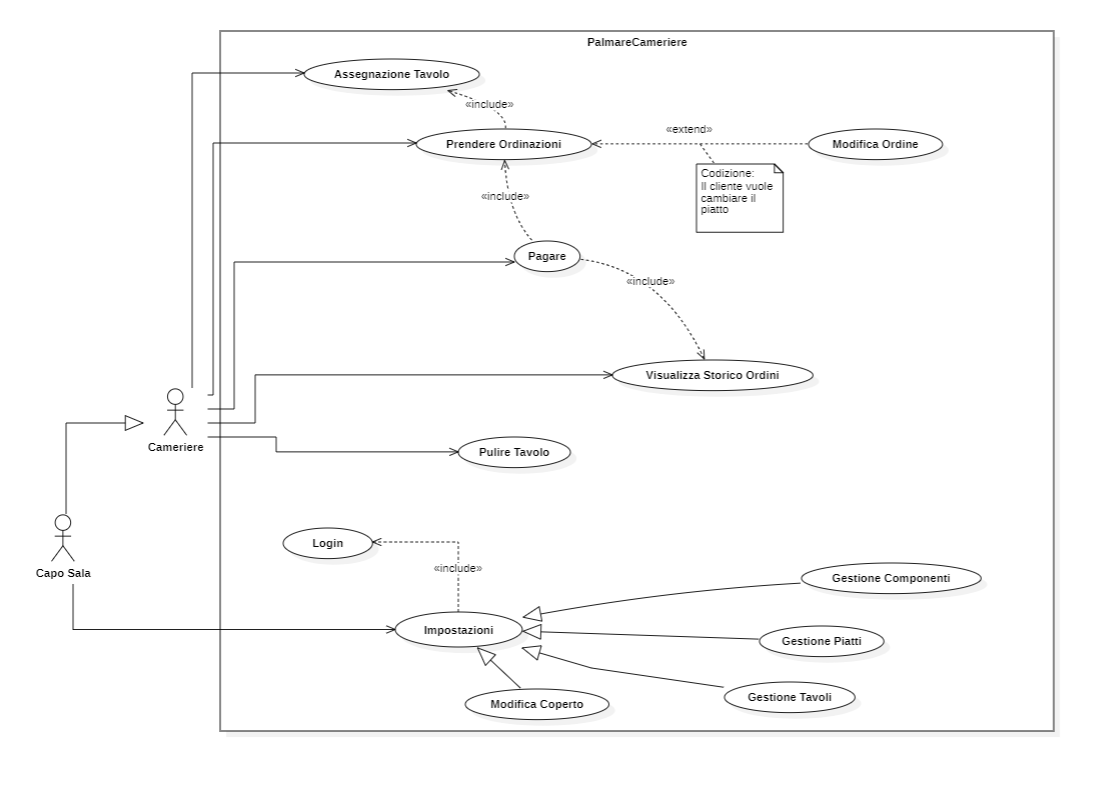
\includegraphics[width=1\linewidth]{../../UML/Diagrammi/Use_Case_Diagram.png}
%     \caption{Use Case Diagram}
%     \label{fig: use_case_diagram}
% \end{figure}

\end{document}